% ABOUTME: The five-stage pipeline: partitioning, pipeline registers, hazard and forwarding units.
% ABOUTME: Owner: Sarvesh (with Aryan for the datapath and control partitioning).
\section{Proposed Solution: Five-Stage Pipeline}
\label{sec:pipeline}

\begin{figure*}[t]
\centering
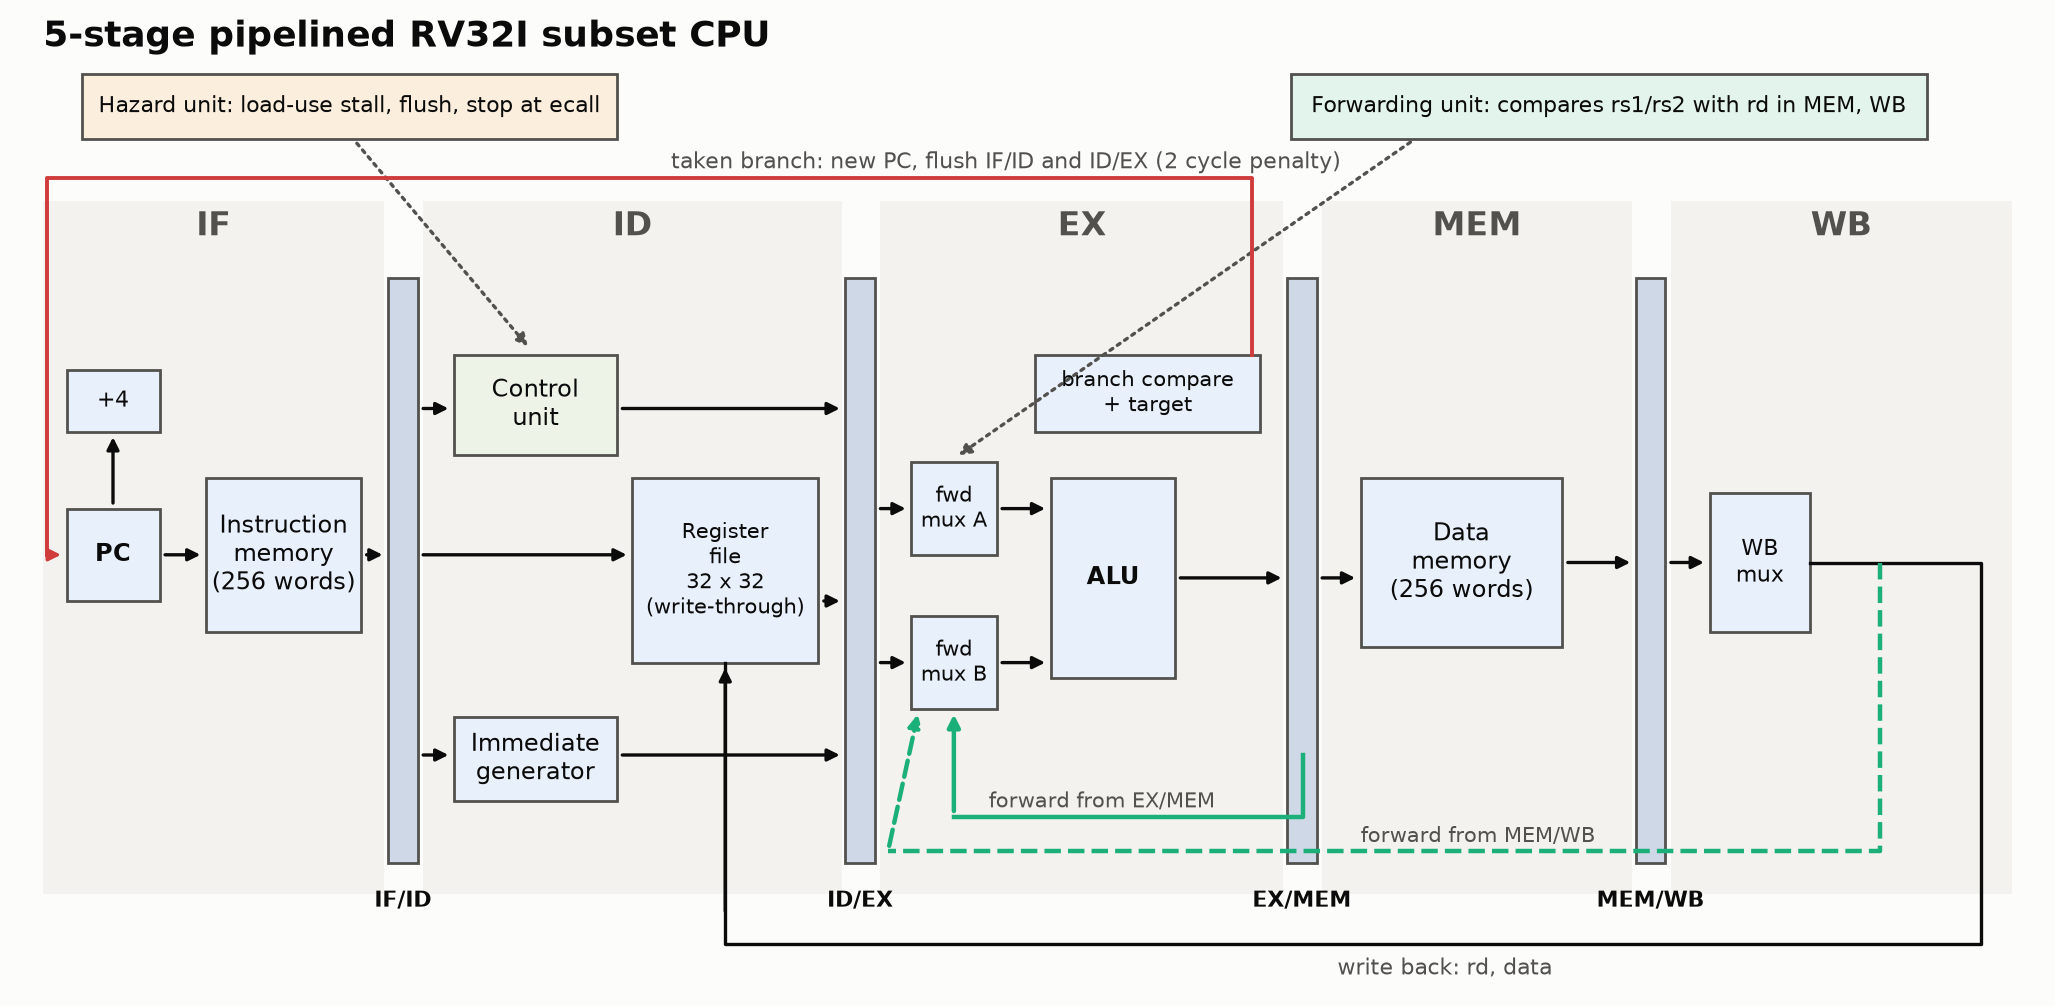
\includegraphics[width=\textwidth]{architecture_pipeline.png}
\caption{Datapath of the pipelined CPU. Grey bars are pipeline registers.
Green paths forward results to the ALU inputs; the red path redirects the PC
and flushes the two younger instructions on a taken branch.}
\label{fig:arch}
\end{figure*}

\subsection{Partitioning}
We cut the verified single-cycle datapath at four points
(Fig.~\ref{fig:arch}), one Verilog module per stage and per pipeline register,
following the brief: \texttt{if\_stage} (PC and instruction memory),
\texttt{id\_stage} (control unit, immediate generator and register file),
\texttt{ex\_stage} (forwarding muxes, ALU, branch comparator and target),
\texttt{mem\_stage} (data memory) and \texttt{wb\_stage} (write-back mux).
\texttt{cpu\_pipeline.v} only wires them together. Datapath and control are
partitioned the same way: control signals are decoded once in ID and travel
with their instruction through the pipeline registers, and each stage uses
only the signals it needs.

\subsection{Pipeline registers}
Table~\ref{tab:pregs} lists what each register carries. Every register
holds a \texttt{valid} bit, so a bubble is an ordinary entry with
\texttt{valid}=0 and all control bits zero. The PC travels with each
instruction because EX needs it for the branch target; the copies in later
stages exist for tracing and are removed by synthesis.

\begin{table}[t]
\centering
\caption{Pipeline register contents}
\label{tab:pregs}
\begin{tabular}{@{}lp{5.3cm}@{}}
\toprule
Register & Fields \\
\midrule
IF/ID & valid, PC, instruction \\
ID/EX & valid, PC, rs1 and rs2 values, immediate, rs1, rs2 and rd numbers,
RegWrite, ALUSrc, MemRead, MemWrite, Branch, BranchNe, Halt, ALU op \\
EX/MEM & valid, PC, ALU result, store data, rd, RegWrite, MemRead, MemWrite,
Halt \\
MEM/WB & valid, PC, ALU result, loaded word, rd, RegWrite, MemRead, Halt \\
\bottomrule
\end{tabular}
\end{table}

A flush clears only \texttt{valid} and the control bits, as in the textbook
design \cite{patterson2021}; data fields of a bubble are never used. Our first
version also cleared every data field. That put a synchronous reset on about
140 flip-flops at the end of the branch flush path, the slowest path of the
forwarding pipeline. Clearing control only raised its Fmax from 76.2 to
83.9\,MHz with no change in behaviour.

\subsection{Register file timing}
The register file is written at the end of WB and read in ID. When an
instruction in ID reads the register that WB is writing in the same cycle,
the register file returns the value being written (write-through). This is the
hardware form of the textbook ``write in the first half, read in the second
half'', and it removes the hazard at distance three without any forwarding
path. The single-cycle CPU must not have this bypass: there the write data
depends on the read data, and the bypass mux forms a combinational loop, which
Yosys reported on our first synthesis run. A Verilog \texttt{generate} block
builds the bypass only when the parameter asks for it.

\subsection{Forwarding unit}
For each ALU operand the forwarding unit compares the source register of the
instruction in EX with the destination of the instructions in MEM and WB:
\begin{equation*}
\mathit{fwdA} =
\begin{cases}
\text{EX/MEM} & \text{if } \mathit{RegWrite}_{M} \wedge rd_{M} = rs1_{E},\\
\text{MEM/WB} & \text{else if } \mathit{RegWrite}_{W} \wedge rd_{W} = rs1_{E},\\
\text{register file} & \text{otherwise,}
\end{cases}
\end{equation*}
and the same for operand B with $rs2_{E}$. EX/MEM wins because it holds the
newer value when both match. \textit{RegWrite} is already 0 when $rd$ is
x0, so a write to x0 is never forwarded. The forwarded operand B is also the
store data, so a store can save a value computed by the instruction just
before it. Setting the parameter \texttt{FORWARDING} to 0 ties both selects
to ``register file'', which gives the second pipeline in our comparison.

\subsection{Hazard unit}
With forwarding, the only data hazard that must stall is a load followed
at once by a use of its result:
\begin{align*}
\mathit{loadUse} = {} & \mathit{MemRead}_{E} \wedge \mathit{RegWrite}_{E} \\
& \wedge \big( (\mathit{usesRs1}_{D} \wedge rs1_{D} = rd_{E}) \\
& \quad \vee (\mathit{usesRs2}_{D} \wedge rs2_{D} = rd_{E}) \big).
\end{align*}
The \textit{usesRs} flags come from the control unit, so immediate bits that
look like a register number never cause a stall. Without forwarding, the unit stalls whenever the
instruction in ID reads the destination of the instruction in EX or MEM.
A stall holds the PC and IF/ID and turns ID/EX into a bubble.

A taken branch is resolved in EX. The PC loads the target, and IF/ID and
ID/EX are flushed, which discards the two instructions fetched on the wrong
path. A flush takes priority over a stall, because the stalled instruction
is itself on the wrong path.

\subsection{Stopping at \texttt{ecall}}
The pipeline fetches instructions behind \texttt{ecall} before it reaches
WB, and a store among them would change memory. When \texttt{ecall} leaves
ID (and is not being flushed), the hazard unit freezes the PC and feeds
bubbles into IF/ID from then on. The program ends when \texttt{ecall}
reaches WB, after every older instruction has completed.
